
\begin{center}
    \textsc{Paragraph For Questions 13 \& 14}
\end{center}

A spray gun is shown in the figure where a piston pushes air out of a nozzle. A thin tube of uniform cross section is connected to the nozzle. The other end of the tube is in a small liquid container. As the piston pushes air through the nozzle, the liquid from the container rises into the nozzle and is sprayed out. For the spray gun shown, the radii of the piston and the nozzle are $20\: \text{mm}$ and $1\: \text{mm}$, respectively. The upper end of the container is open to the atmosphere.

\begin{center}
    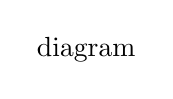
\begin{tikzpicture}
    \node {diagram};     
\end{tikzpicture}
\end{center}

\item If the piston is pushed at a speed of $5\: \text{mm s}^{-1}$, the air comes out of the nozzle with a speed of
    \begin{tasks}(4)
        \task {$0.1\: \text{m s}^{-1}$}
        \task {$1\: \text{m s}^{-1}$}
        \task {$2\: \text{m s}^{-1}$}
        \task {$8\: \text{m s}^{-1}$}
    \end{tasks}

\item If the density of air is $\rho_a$ and that of the liquid $\rho_e$, then for a given piston speed the rate (volume per unit time) at which the liquid is sprayed will be proportional to
    \begin{tasks}(4)
        \task {$\sqrt{\frac{\rho_a}{\rho_e}}$}
        \task {$\sqrt{\rho_a \rho_e}$}
        \task {$\frac{\rho_e}{\sqrt{\rho_a}}$}
        \task {$\rho_e \rho_a$}
    \end{tasks}
